\documentclass[]{article}
\usepackage{mathtools}
\usepackage{graphicx}
\usepackage{hyperref}
\usepackage[]{algorithm2e}

%opening
\title{Visualizing Graduate Admissions Data \\ CMPS 161: Final Project}
\author{Aaron Doubek-Kraft \\ adoubekk@ucsc.edu}
\date{March 20, 2017}



\begin{document}


	
\begin{titlepage}

	\maketitle

	\begin{abstract}
		The unusually large applicant pool to the Computer Science graduate program at UCSC in 2017 introduced a problem of scale to the admissions process. By applying multivariate visualization techniques to applicants' admission data, I aim to identify correlations in the data that could be applicable to the selection process in the future. I employ a common information visualization technique known as the parallel coordinate plot. A brief overview of this technique is provided, as well as descriptions of several common methods to improve its readability and usefulness that are implemented in this project.
	\end{abstract}

\end{titlepage}

\section{Introduction}

	\par In 2017, there were nearly 1100 applicants to the UC Santa Cruz Computer Science graduate program. Given the unusually large size of this applicant pool, making sense of any large-scale trends simply by looking at their records in a table becomes an intractable problem. In addition to the high volume of applicants, the students' records contain a large number of potentially significant variables to be analyzed. This includes quantitative data, such as test scores and GPA, and qualitative data, such as the applicants' research interests, countries of origin, and whether or not the student was admitted.  In this paper, I attempt to develop visualizations to identify correlations in this data that could be relevant to the selection process. 

\section{Methods}

	The large number of variables and the high volume of records to be analyzed makes this a classic multivariate visualization problem, and so I take a relatively standard approach: the parallel coordinate plot. In a typical graph, the number of variables available to be displayed is limited to two or three, the number of spatial dimensions, so only correlations between a relatively small number of variables may be analyzed at a time (for example, in a scatter plot). The parallel coordinate plot generalizes the graphical approach to an arbitrary number of axes, allowing correlations to be analyzed across a large number of variables.

	\begin{figure}[h]
		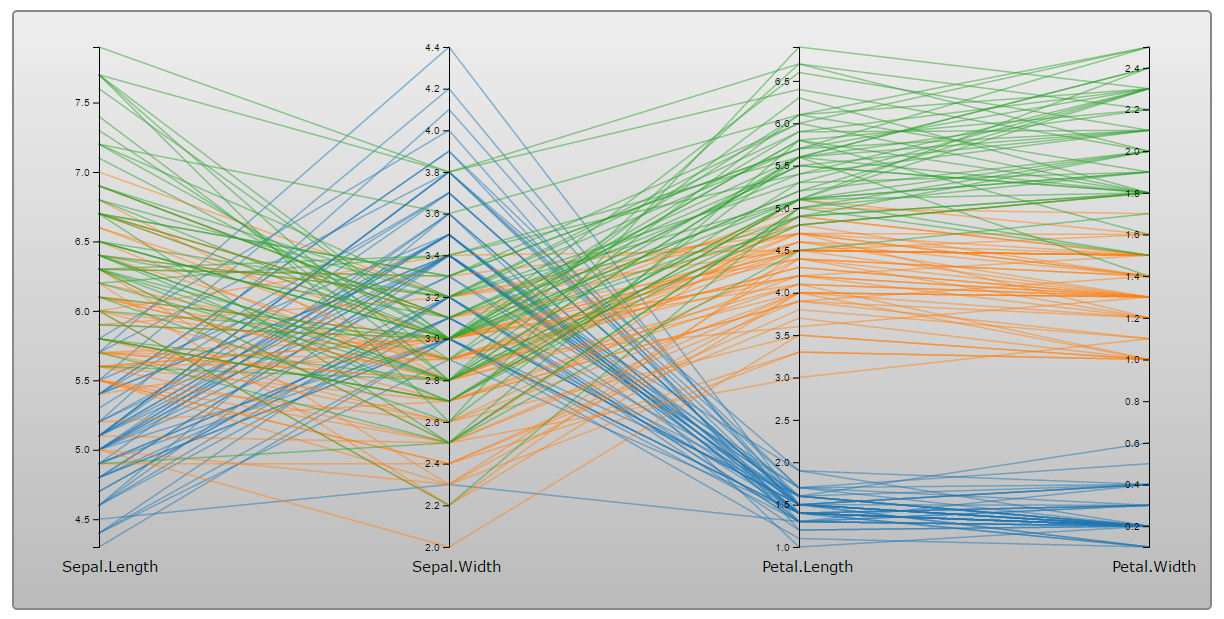
\includegraphics[width=\linewidth]{iris.png}
		\caption{Visualizing Edgar Anderson's Iris dataset. In this example, color is mapped to species of iris.}
		\label{fig:Result}
	\end{figure}
	
	\par As an example, I present a standard test case for multivariate visualization: the iris dataset.\cite{datasets} Even in the absence of any specific knowledge about irises, some trends are immediately apparent. First, petal length and petal width are clustered for a given species, and they appear to be directly correlated: irises either have large petals or small petals. Similarly, sepal length and sepal width are also clustered, though not as strongly as petal size, and they appear to be inversely correlated (in case the reader is curious, the sepals are the green parts outside the flower that protect the petals, a fact I had to look up). Using the high dimensionality, we can compare axes across the chart, and we can see that sepal length is also correlated to petal width. Now, the strength of this approach becomes clear: it would have taken four or five lower-dimensional charts such as scatterplots to reach the same conclusions that are presented here in one condensed figure. I leave analyzing the significance of these trends to the botanists.
	
	\par The parallel coordinate plot, in its most basic form, also has the advantage of simplicity: straight lines connecting parallel axes are not difficult to implement, especially given the powerful scaling and rendering functionality of the d3.js library\cite{d3} used in this project. The challenge is in scaling the visualization up to larger datasets. The iris dataset consists of only 150 records, while the graduate admissions data has almost 1100, so approximately seven times the number of lines will be drawn on the plot. Without some additional adjustments, the plot will be too visually cluttered to be of any use. One simple technique to improve readability is to map the color of the lines to their group membership, as color is mapped to species in the iris example. I will discuss additional techniques in the Implementation section.
	
\section{Implementation}
	\subsection{Dataset: Description and Processing}
		The dataset consists of 1097 records, each representing an applicant to one of the UCSC computer science graduate programs. The fields from the provided dataset are described as follows:
		
		\begin{tabular}{c|c}
		 Field & Description \\ \hline
		 ID & Applicant identification number \\
		 Tags & Filters and Professors' interest in applicant\\
		 Transcripts Rec'd & Number of transcripts received \\ 
		 Transcripts Req'd & Number of transcripts required \\
		 Letters Rec'd & Number of recommendation letters received\\
		 Dept & Academic Department (all CMPS)\\
		 Degree & Masters or PHD\\
		 Research Interests & Applicant's list of research interests\\
		 Schools Attended & Applicant's previous education\\
		 UG GPA & Undergraduate GPA\\
		 UG GPA SCALE & Scale for undergraduate GPA\\ 		 
		 GRAD GPA & Graduate GPA\\
		 GRAD GPA SCALE & Scale for graduate GPA\\
		 GREV & GRE - Verbal Reasoning\\
		 GREV\% & Percentage of total possible GREV score\\
		 GREQ & GRE - Quantitative Reasoning\\
		 GREQ\% & Percentage for GREQ\\
		 GREA & GRE - Analytical Writing\\
		 GREA\% & Percentage for GREA\\
		 GRESubjName & GRE Subject Test Name \\ 
		 GRESubjScore & Gre Subject Test Score\\
		 GRESubj\% & Gre Subject Test Percentage\\
		 TOEFL & Test Of English as a Foreign Language\\
		 IELTS & International English Language Testing System \\
		 Gender & Male, Female, Other, or Unreported\\
		 Ethnicity & \\
		 CA Res & California Resident: Yes, No, or Unreported\\
		 For/Dom & Domestic, or Country of Origin\\
		 Number of Reviews & \\ 
		 Ratings & \\ 
		 Avg. Rating & \\ 
		 Admitted & Yes or No\\
		\end{tabular} \\
		
		\par Since the applicants come from all around the world (in fact, the vast majority of applicants were foreign), one obstacle to drawing objective quantitative comparisons between groups of students was the fact that not all students have taken the same tests, and GPA is scaled differently in different countries. Normalizing the GPAs was relatively straightforward, since the dataset includes both the student's GPA and the GPA scale used, so the scores were simply normalized to 1, or in other words, the fraction of the appropriate total possible GPA. Additionally, a small number of the reported GRE scores were far higher the actual maximum score on the exam\cite{GRE}, so these were simply thrown out. Finally, there are two different English as a Foreign Language exams, the TOEFL\cite{TOEFL} and the IELTS\cite{IELTS}. These two were merged into a single EFL Index, again by normalizing to the maximum score on each exam. However, these two exams are score quite differently: TOEFL reports a score in the range 0-120, while IELTS assigns a "band" from 0-9 based on proficiency. A more representative comparison might be to fit each set of scores to a distribution, but there were relatively few IELTS scores, so this approach may also have introduced some bias as well. \\
		
		\par The fields I added to the dataset are defined as follows: \\
		
		\begin{tabular}{c|c}
		Field & Description \\ \hline \\
		UG GPA (Normalized) & $\frac {\text{UG GPA}}{\text{UG GPA SCALE}}$\\ \\
		GRAD GPA (Normalized) &  $\frac{\text{GRAD GPA}}{\text{GRAD GPA SCALE}}$\\ \\
		EFL (Normalized) & $\frac{\text{Score}}{\text{Max Score}}$, for TOEFL and IELTS\\		
		\end{tabular}
		
	\subsection{Developing Visualization}
		\par In this section, I will discuss the strategies implemented in this project to improve readability of parallel coordinate plots of large datasets. While the primary objective here was analysis of the graduate admissions data, the techniques used here, and in fact the interface itself, could be used to visualize any multivariate dataset stored as a csv file. In general, however, csv is a relatively loose standard\cite{csv}, so any truly generic application is nearly impossible.
		\subsubsection{Color Mapping}
			As the interface was designed to be a relatively generic approach to multivariate data, the program will parse potential relevant groups from the dataset itself and color-code them according to group membership. If the dataset contains multiple potential groupings, as the graduate admissions data does, the interface also allows the user to decide which grouping to use. This facilitates comparisons between subsets of the data, as well as identifications of correlations within a particular group.
		\subsubsection{Highlighting}
			If the user is interested only in a certain subset or subsets of the data, those may be selected, and all other subsets will be grayed out. This further emphasizes correlations (or the lack thereof) within this subset.
		\begin{figure}[h]
			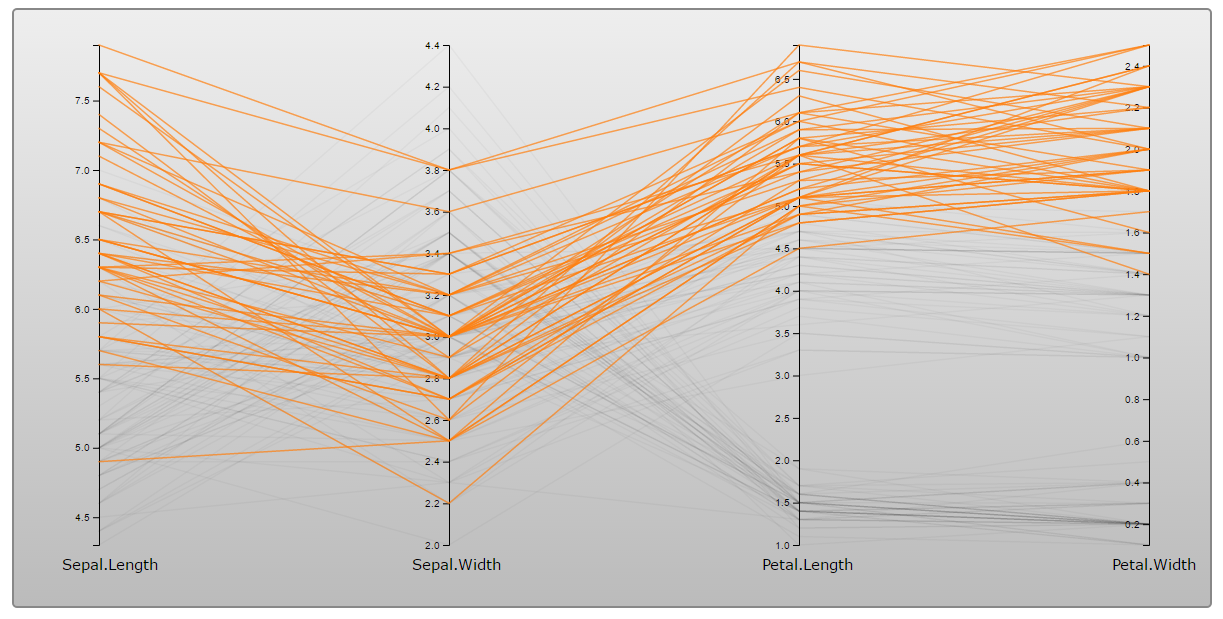
\includegraphics[width=\linewidth/2]{highlight.png}
			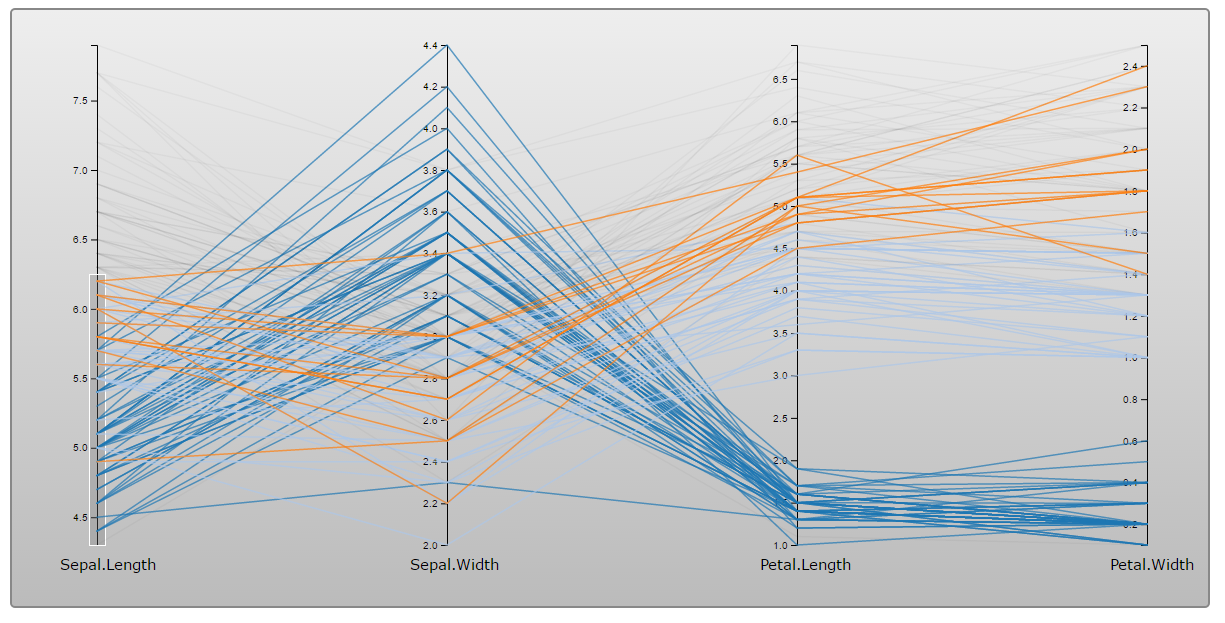
\includegraphics[width=\linewidth/2]{brush.png}
			\caption{Left: Iris dataset, with only species \textit{setosa} highlighted. Right: same dataset, with a brush applied for low sepal width.}
			\label{fig:Brush/Highlight}
		\end{figure}
		\subsubsection{Brushing}
			Brushing involves selecting only those records which fall in a particular range on a given axis \cite{bostock,kosara}, and highlighting the associated polylines. This technique is particularly well suited to identifying correlations in larger datasets, because it allows the user to identify clusters within the data, and track those clusters across the many variables.
			
			\par The algorithm used to determine which lines have been selected is described as follows:\\
			
			\begin{algorithm}[H]
				\SetAlgoLined
				\KwData {d3.js brush objects, which contain currently brushed extent on a given axis, and an array of records}
				\KwResult {an array of booleans indicating whether the line corresponding to that record has been selected}
				
				n = number of records\;
				brushed = array of booleans with size n, initialized to true\;
				\For {each axis} {
					extent = selection area of brush on this axis\;
					\For {each record} {
						datapoint = value of record on this axis\;
						\If{datapoint within extent} {
							brushed[this record] = false\;	
						}
					}
				}
				\Return {brushed}

			\end{algorithm}
		\subsubsection{Axis Selection}
		The visualization interface allows the user to select what axes to be displayed on the plot. While most of the strategies discusses here focus on highlighting clusters or trends in the data, this was implemented as a way to reduce the scale of the problem. For example, variables that take on only a small range of discrete values are typically not suited to this type of visualization\cite{kosara}, so this tool can simply eliminate such variables from the view.
		\begin{figure}[h]
			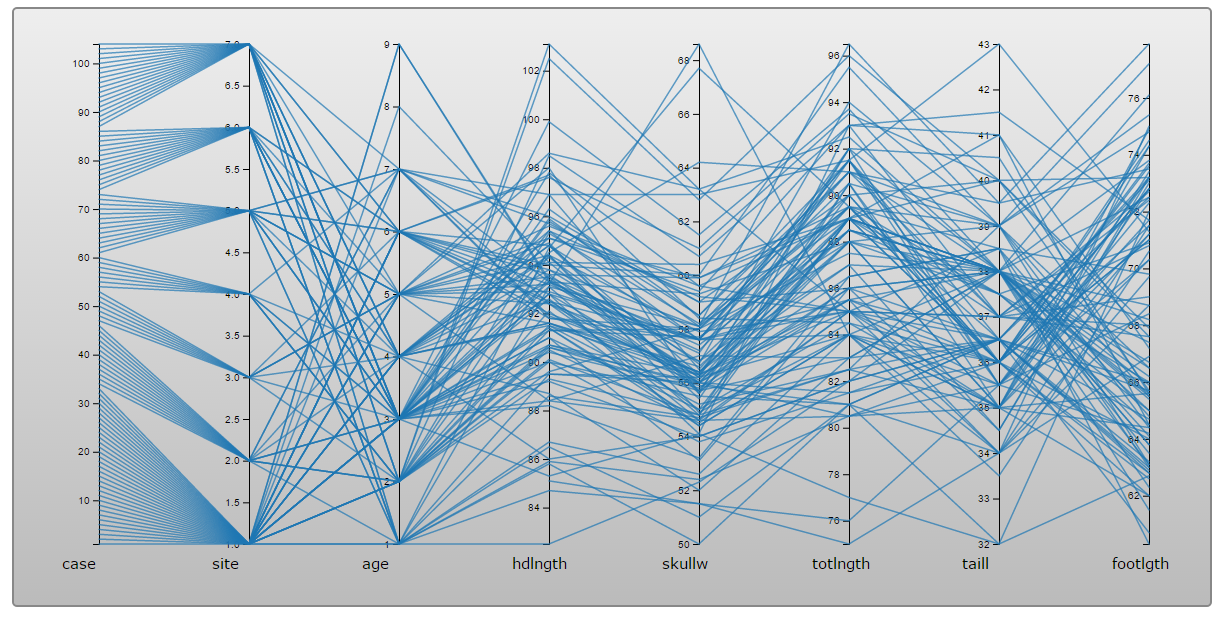
\includegraphics[width=\linewidth/2]{possum_bad.png}
			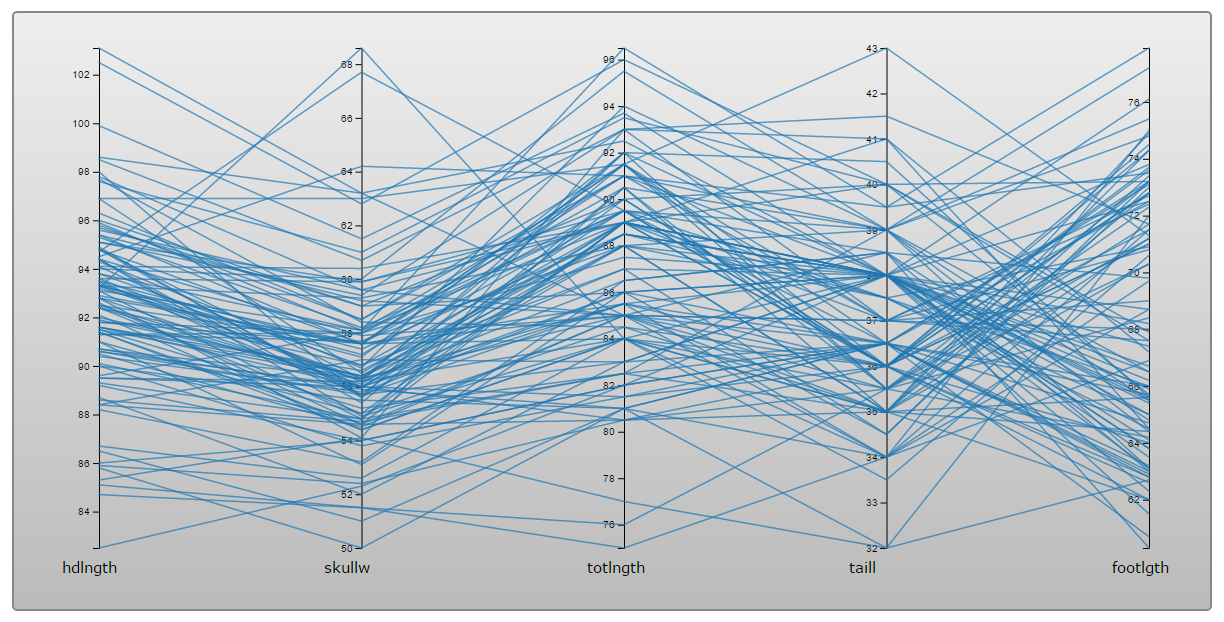
\includegraphics[width=\linewidth/2]{possum_good.png}
			\caption{Left: Possum dataset\cite{datasets}, with discrete variables on left axes. Right: same dataset, with discrete variables eliminated using axis selection.}
			\label{fig:Axis}
		\end{figure}
	\subsection{Technical}
		This project uses d3.js 4.7.3 to handle the rendering of the visualizations (modules: d3-axis, d3-scale, d3-selection, d3-brush, and d3-shape), jQuery.js for DOM manipulation and user input, w3.css as a style framework, and Python scripts for dataset processing tasks. The data is read into Record objects, each of which contains two native JavaScript maps: one from keys to values for qualitative data (defined as "sets" or "groups" in the code) and one from keys to quantitative (defined as "data"). These record objects also define getter and setter functions, although this is mainly a matter of convenience as JavaScript does not provide a robust system of encapsulation.
\section{Results}
	In my original implementation, the lines that were not selected were simply grayed out. This made for a nice visual effect on smaller datasets, but on the graduate admissions dataset, the plot was simply too densely populated, and even the greyed out lines became a visual distraction and hindrance. For the graduate admissions data, this effect was disabled.

	\begin{figure}[h]
		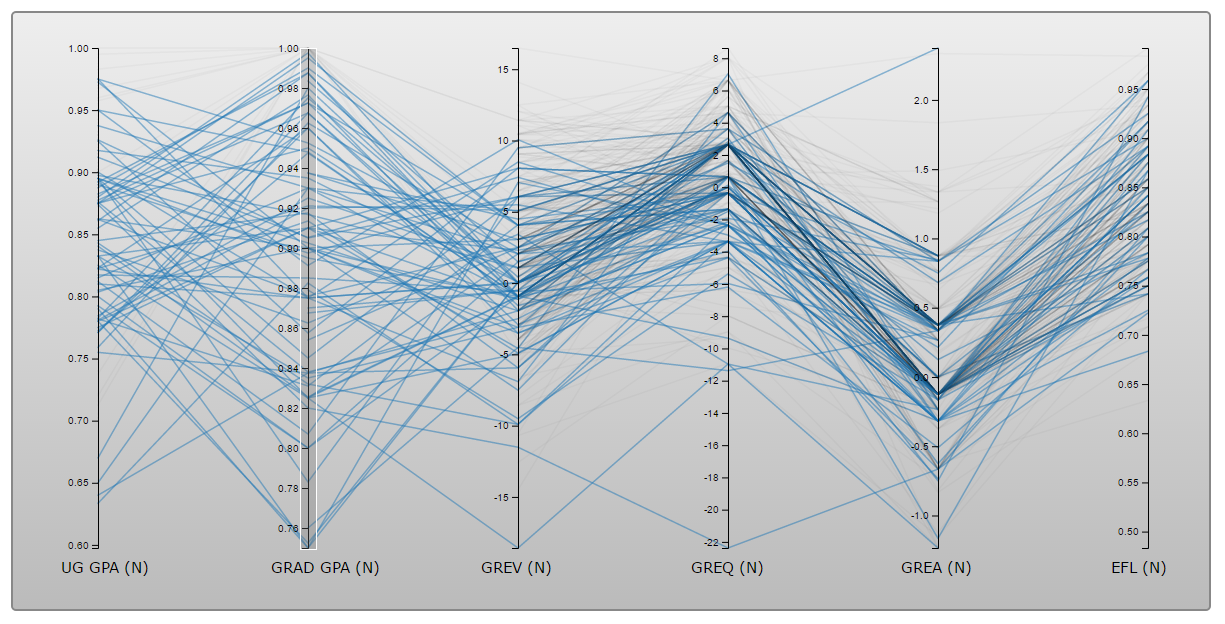
\includegraphics[width=\linewidth]{grads_only.png}
		\caption{Graduate admissions dataset, brushed along the GRAD GPA axis (i.e. showing only those students who had previously attended graduate school). Color mapped to CA residency: Blue = Non-resident, Orange = Resident}
		\label{fig:Grad}
	\end{figure}
	
	Interestingly, in this Figure 4, it appears that students who had previously attended graduate school had relatively low GRE - Verbal Reasoning and Analytical Writing scores. Applying the appropriate color map to this plot clarified the situation, however. The vast majority of these students (blue) are non-California residents (in fact, most are foreign, but that mapping contains country of origin and is much more difficult to parse), and it is not a huge surprise that foreign students did not perform as well on an English language verbal proficiency test than did native speakers.
	
	
\section{Related Work}
	Parallel Sets, Radviz (time permitting)
	
\section{Conclusion}
	There is a great deal of potential for improvement of this interface. In order to be a useful generic tool, many more of the visual attributes of the graph could be customizable, including the colors of the lines, whether unselected lines are grayed out or hidden, how and where the labels are placed, etc. In addition, there are several features I planned to implement but couldn't fit in before the deadline. First, I planned to allow switching from the quantitative "data" category to the qualitative "sets" category, as some discrete variables (such as store number, number of letters received, etc.) could be more useful as groupings than as plotted data.

\vfill

\begin{thebibliography}{11}
	\bibitem{bostock}
		Bostock, Mike. Parallel Coordinates Example [Internet]. d3.js; Available from \url{http://mbostock.github.io/d3/talk/20111116/iris-parallel.html}
	\bibitem{csv}
		Comma Separated Values (CSV) Standard File Format [Internet]. Edoceo. Available from \url{http://edoceo.com/utilitas/csv-file-format}
	\bibitem{d3}
		d3.js: Data Driven Documents. Available from \url{https://d3js.org/}
	\bibitem{GRE}
		GRE Scores [Internet]. Available from \url{https://www.ets.org/gre/revised_general/scores/?WT.ac=grehome_grescores_150213}
	\bibitem{IELTS}
		How IELTS is scored[Internet] https://www.ielts.org/about-the-test/how-ielts-is-scored
	\bibitem{kosara}
		Kosara, Robert. Parallel Coordinates [Internet]. Eagereyes; 2010. Available from \url{https://eagereyes.org/techniques/parallel-coordinates}
	\bibitem{datasets}
		R Datasets [Internet]. Available from: \url{https://vincentarelbundock.github.io/Rdatasets/datasets.html}
	\bibitem{telea}
		Telea, Alexandru C. Data Visualization Principles and Practice. 2nd Edition. Boca Raton(FL): CRC Press; 2015.
	\bibitem{TOEFL}
		TOEFL iBT® Test Scores [Internet]. \url{https://www.ets.org/toefl/ibt/scores}
\end{thebibliography}


\end{document}